% Chapter 3

\chapter{Lumped parameters modelling in Munadarnes geothermal system } % Main chapter title

\label{Chapter3} % For referencing the chapter elsewhere, use \ref{Chapter1} 

\lhead{Chapter 3. \emph{Lumped parameter modelling with case study}} % This is for the header on each page - perhaps a shortened title

%----------------------------------------------------------------------------------------


%----------------------------------------------------------------------------------------
\section{Munardanes low temperature system}

\begin{figure}[H] %  figure placement: here, top, bottom, or page
   \centering
   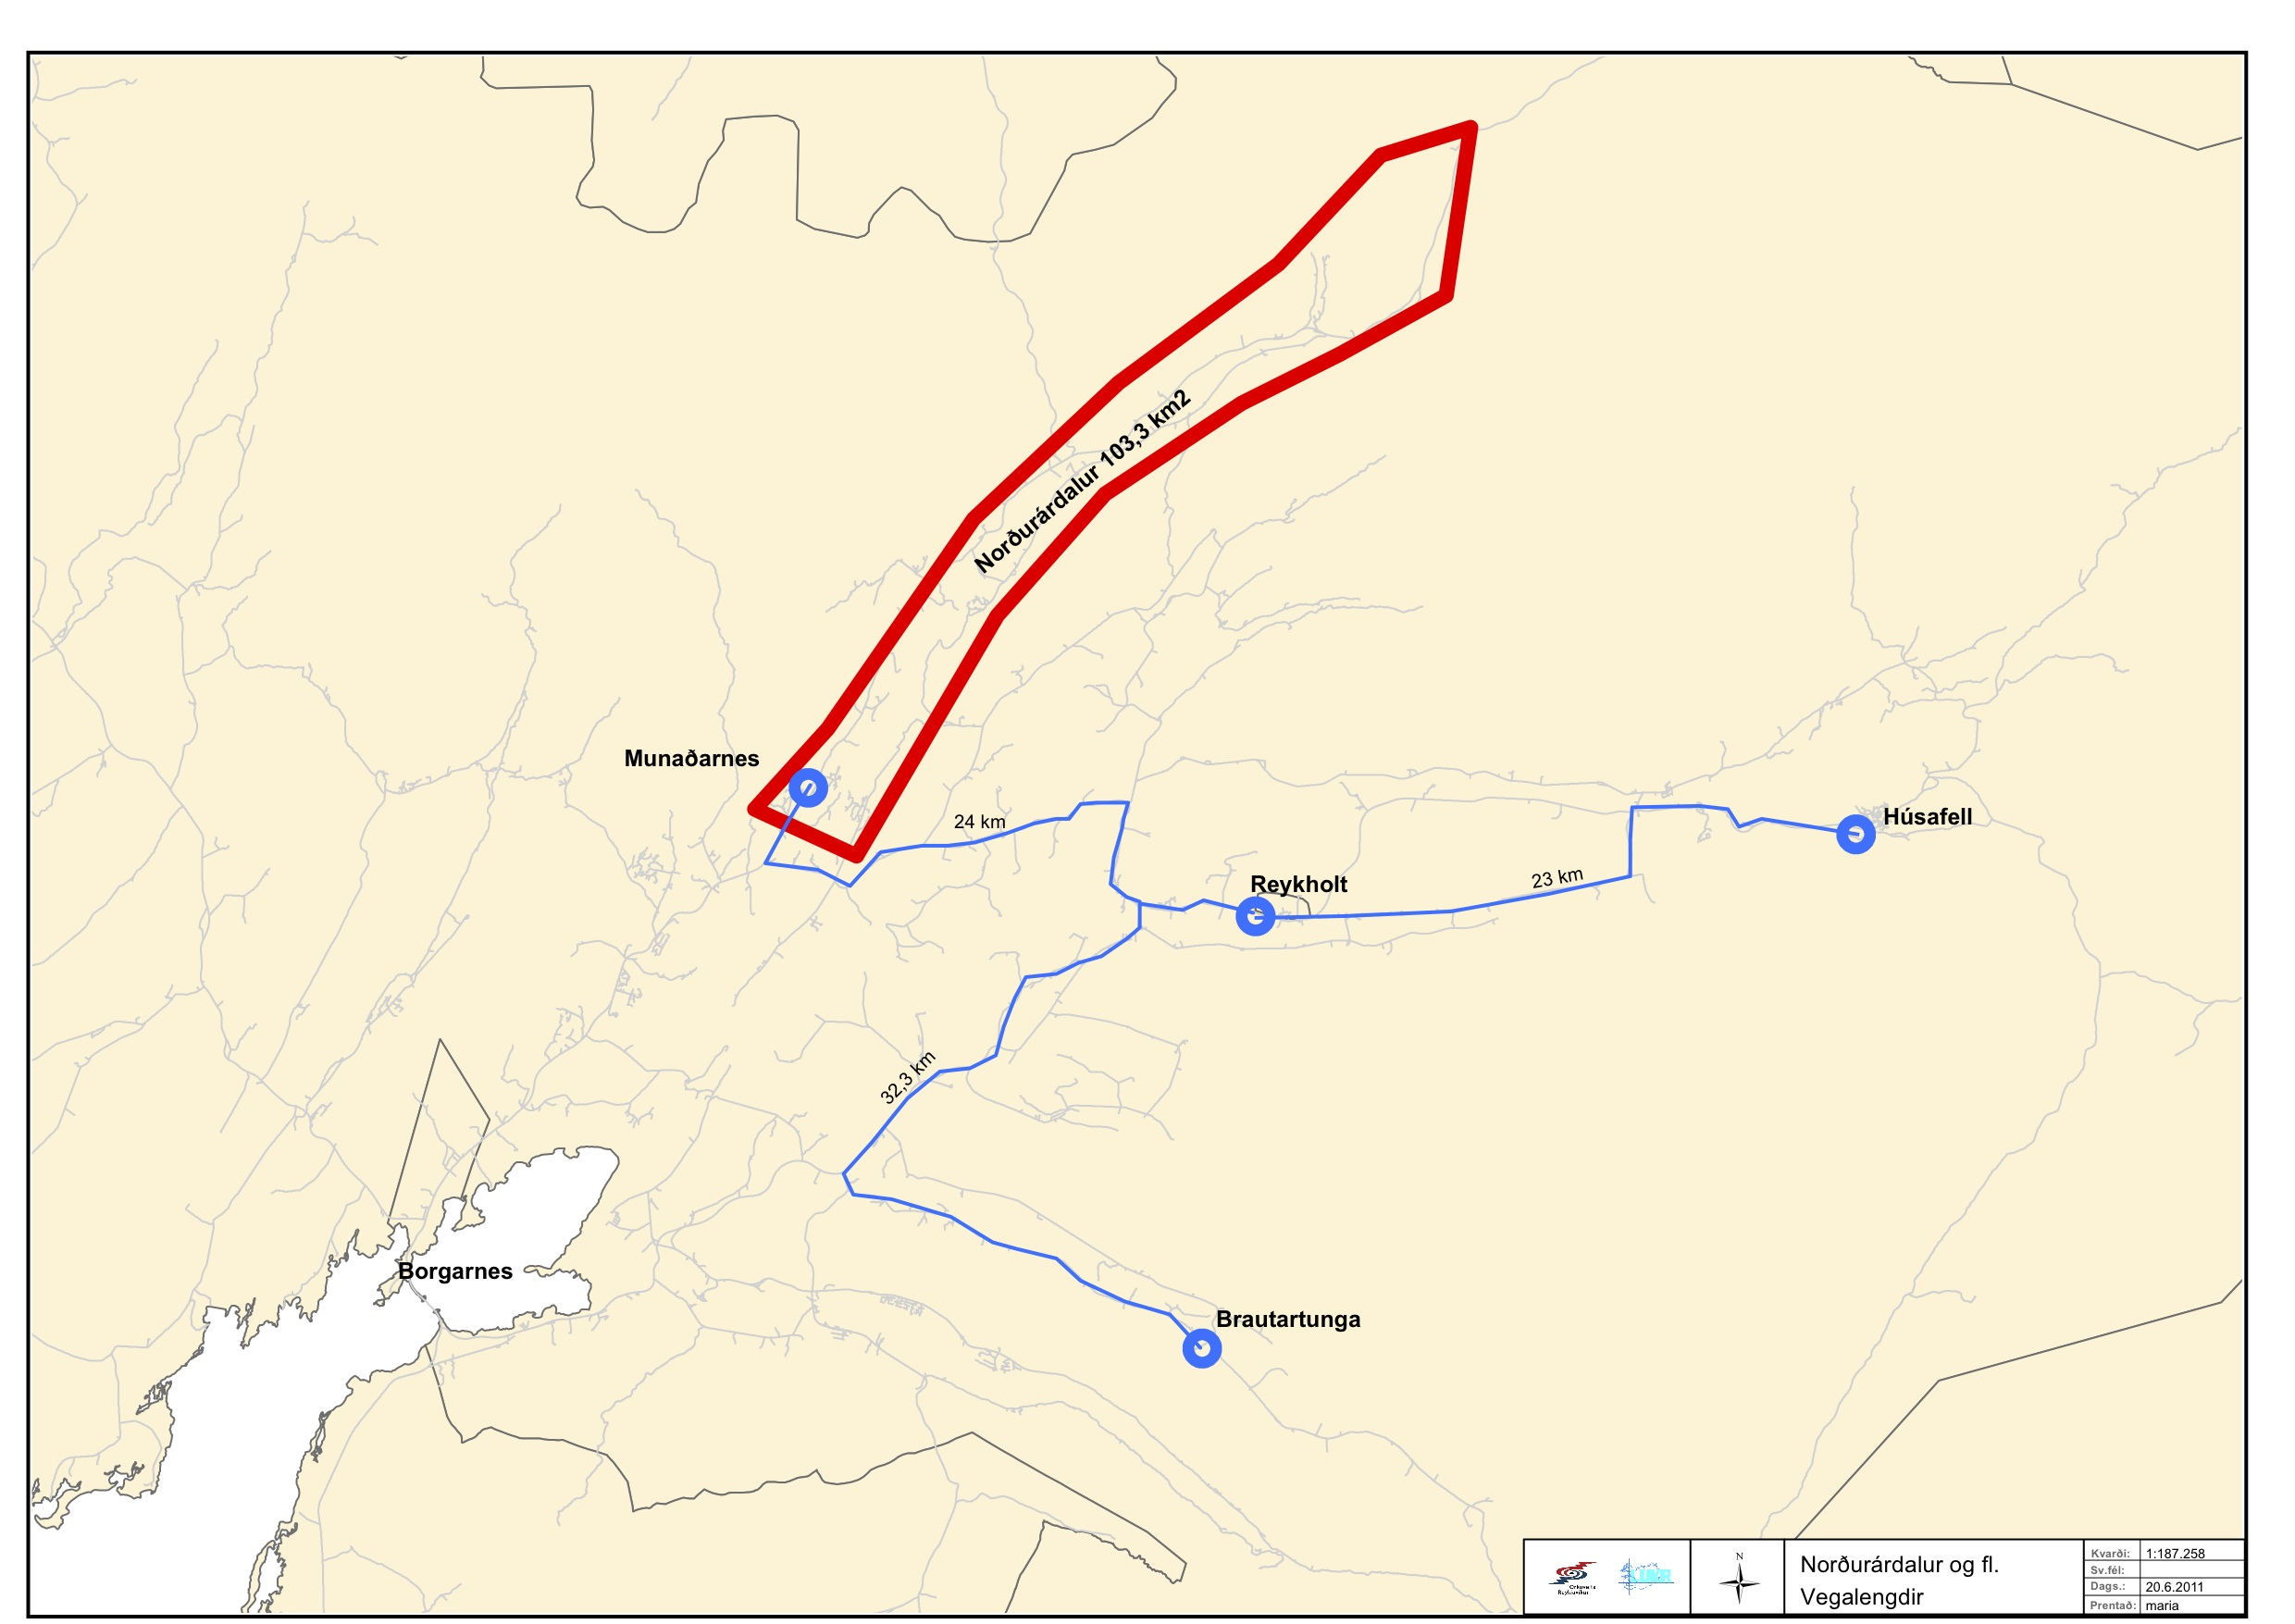
\includegraphics[width=5in]{nordu.jpg} 
   \caption{ Borgarfjordur thermal field and Nordurardalur thermal system}
   \label{fig:nordu}
\end{figure}
The Munardanes reservoir is situated in the Nordurardalur geothermal field. The later is located in west Iceland in the Borgarfjordur thermal field situated in the Borgarfjordur region. The Borgarfjordur thermal field is the largest low temperature geothermal field in Iceland. It comprises known thermal systems such as the Reykholt thermal system, the Bear thermal system, the Brautartunga thermal system, England thermal system, and the Husafell thermal system (Johannesson et al. 1980, Gunnlaugsson 1980). The natural discharge of the Borgarfjordur thermal system also called the Reykholtsdalur thermal system is estimated to 450$l/s$ of boiling water (Georgsson et al. 1984).  Within the Borgarfjordur thermal field, the Reykholf thermal system is by fare the largest thermal system with a total discharge of 400$l/s$ (Georgsson et al. 1980). The Nordurardalur thermal system is located north-west to the five major thermals systems mention above. It is a N-W long band of about 103 $km^{2}$ .

\subsection{Geological setting}
\begin{figure}[H] %  figure placement: here, top, bottom, or page
   \centering
   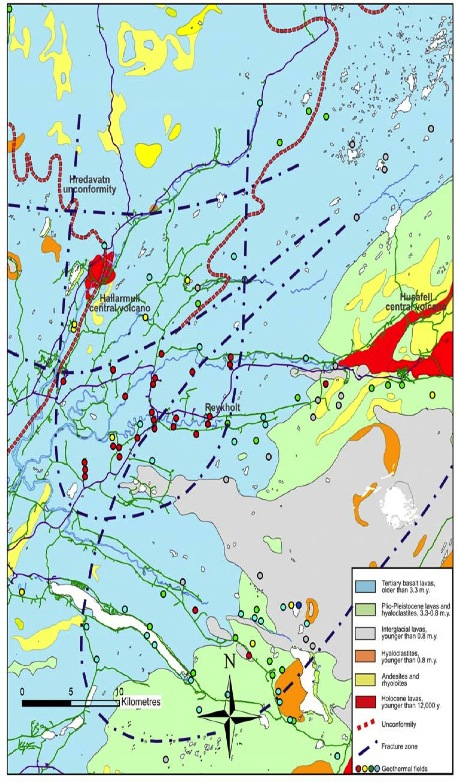
\includegraphics[width=4in]{bgeo.jpg} 
   \caption{Geological map of Borgarfjordur thermal field}
   \label{fig:bgeo}
\end{figure}

Upper tertiary ($>$3.3 Myr) basaltic lava flow constitute the basement of the Borgarfjordur region. This lava flow is characterised by a uniform lithology, either uniform texture or composition. The oldest rock being 14-15 Myrs. The bulk of this tertiary lava flow is made of tholeiites basaltic rock separated by minor clastic interbeds (Saemundsson, 1979). The tholeiites basaltic lava pile is characterized by its content in sodium which is less than other basaltic rock. The Borgarfjordur thermal field is bounded from the east by the western volcanic rift zone and the snaefellnes volcanic zone from the west. The later present little or no rifting. Those two volcanic zones represent the origin of the tertiary lava flow.  However, the tholeiites content of the lava flow suggest that the lava flow is predominantly from the Sneafellsnes volcanic flank zone. \\
\\
 Both unconformity and anticline structures are visible in the region. The later formed from rift relocation (Saemundsson, 1967). Recall that an anticline is defined as layers of sedimentary rock having the oldest strata in its core and forming a convex shape. An unconformity is a planar structure indicating a discontinuity in a geologicale structure due to erosive forces. The anticline axis is defined as the line of intersection of the perpendicular plane cutting the anticline in two symmetric parts. The Borganes anticline runs NE-SW (saemundsson, 1977). The lava flow dip towards the Reykjanes-Langjokull rift zone to the east of the anticline axis. The Hredavatn unconformity is situated in north of Hredavatn lake. This unconformity indicate intense erosive forces acting in the borgarfjordur region.

\subsection{Geophysical and hydrological setting}

The geophysics of the region is characterised by the volcanism, the tectonic and the different forces affecting the earth crustal structure. The region is located between the Sneafellsnes volcanic flank and the Reykjanes-Langjokull volcanic rift. The later is made of the Reykjanes peninsula and the Western volcanic zone. The Reykjanes-Lanjokull rift is characterised by faulting resulting from tensional stress in the earth crust.  The Nordurardalur geothermal system is confined within the WNW-ESE, N-S  fractures zone   and between the Hradavatn unconformity and the Borganes anticline. An extinct central volcano is sitting within the Nordurardalur thermal system.\\
The resistivity in Nordurardalur alternate between 20 and 100 $\Omega m$.  The 20 $\Omega m$ resistivity part is located in the lowest part of the Nordurardalur band and quickly 
increase to 60 and 100 as we move North east. The value alternate to 30-40 then decrease to 20 before increasing to about 30 $\Omega m$.\\
\\
The geothermal water is of meteoric origin which as fallen as precipitation on the highland. The water percolate through fractures cracks or others pathways through the earth and is heated by regional heat flow. The flow pattern can be infer base on preview studies done in the main thermal systems in Borgafjordur. The Northeasterly faults are the main channels for the Nordurardalur thermal system and the seismicity in the region allows fractures to serve as flow path. The recharge zone is the Arnarvatnsheidi highland and the flow pattern is 

\subsection{Proposed conceptual model of Borgarfjordur thermal filed}
\begin{figure}[H] %  figure placement: here, top, bottom, or page
   \centering
   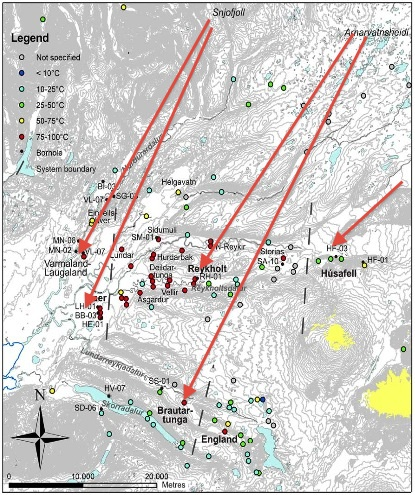
\includegraphics[width=5in]{flowp.jpg} 
   \caption{Production well in Borgarfjordur thermal field with flow patterns of the main thermal systems}
   \label{fig:flowp}
\end{figure}
Figure (\ref{fig:flowp}) indicates the flow patterns of the main thermal system in Borgarfjordur thermal field. The Reykholt and the Brautartungar thermal field recharge zone is located in the Arnarvatnsheidi high land. The Husafell thermal system recharge zone is located east to the Arnarvatnsheidi high land. For those tree systems, the easterly and north easterly faults and fractures allows the meteoric water to percolate at depth, acting as flow channels. The Nordurardalur system can be seen as a part of the Bear thermal system. The recharge zone is situated in the surrounding  of Snjofjoll, latitude 64 Degree 59 $mn$ $N$, longitude 21 Degree 11 $mn$ W. The $NS$ fractures act as flow channels, where the water flows by the Hallarmuli extinct central volcanoes. \\
\\
Heat is transfer by conduction through the earth crust from the Snaefellsnes volcanic flank and the Reykjaness-Langjokull volcanic rift zone. Heat is convected by the hot water though the fracture and fault systems at depth. The integrity of the fracture/fault system are maintain by the seismicity in the region. They also act as barriers zone. The salinity of water is the highest in the Bear thermal system as well as in the Nordurardalur system. As we move away from the Bear system the salinity decreases, being the lowest in Husafell thermal system.


%%%%%%%%%%%%%%%%%%%%%%%%%%%%%%%%%%%%%%%%%%%%%%%%%%%%%%%%


\section{Lumped parameter modelling }
Lumped parameter modelling is a cost effective high precision modelling approach for geothermal systems. It is used to simulate water level or pressure change due to production in a geothermal reservoir. By using a nonlinear iterative least square technique, the computer program LUMPFIT fit automatically the analytical response functions of lumped model to the measured data (water level or pressure), \cite{Ax-Simul-Lump89}. In the lumped model, the geothermal system is represented by tanks, characterised by storage coefficient $\kappa$ and conductor $\sigma$, simulating respectively the  storativity $s$ and permeability $K$. In this modelling process the reservoir is divided into three parts if necessary. For two dimensional flow as in this work, the fluid turbulence coefficient is neglected.

\begin{figure}[htbp] %  figure placement: here, top, bottom, or page
   \centering
   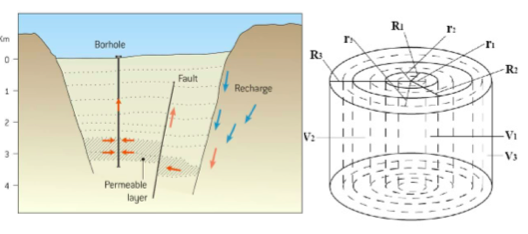
\includegraphics[width=6in]{lump1.png} 
   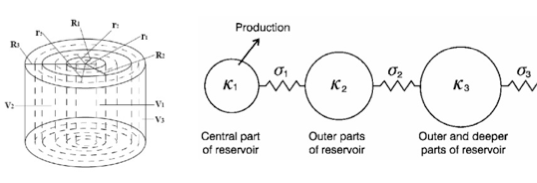
\includegraphics[width=6in]{lump0.png} 
   \caption{Subdivision of the reservoir in recharge, intermediary, and production parts}
   \label{fig:lump1}
\end{figure}

Each part is approximated by a cylindrical tanks with defined radius. The inner cylinder (inner tank) is the production part which is intersected by the production well. Adjacent to inner cylinder is an intermediaries cylinder defining the interface between the recharge part (outer cylinder) and the production part (inner cylinder).  Each cylinder are then approximated by lumped capacitors characterised by the coefficients $\kappa$ and $\sigma$ simulating  storativity $s$ and permeability at the boundary of the cylinder (capacitor).\\
\\
\\
\clearpage
The goal is to fit the theoretical  pressure response

\begin{equation}\label{eq:c}
 P(t)=�\sum Q\frac{A_{i}}{L_{i}}(1-exp(-L_{i}t))+QBt 
\end{equation}

\begin{equation}\label{eq:o}
 P(t)=�\sum Q\frac{A_{i}}{L_{i}}(1-exp(-L_{i}t)) 
\end{equation}
to a set of measured water level data, for an open system and a closed system respectively. Recall that a geothermal system is open when sufficient fluid flow through it boundaries to allow recharge. The opposite is true for a closed system.

The parameters  $A_{i}, L_{i}$, $B$, are function of $\kappa_{i}$ and $\sigma_{i}$.  After evaluating the unknown parameter ( $A_{i}, L_{i}$, $B$,$\kappa_{i}$ and $\sigma_{i}$ ), equations (\ref{eq:c}, \ref{eq:o}) can be used to simulate and predict water level change in time. The size $A$, the depth $H$, the approximate permeability $K$, the storativity $s$ and the  recharge mechanism of the reservoir can also be evaluated and understood using
\begin{equation}
\kappa_{i}=V_{i}s=A_{i}Hs \\
\end{equation}

\begin{equation}
K=\sigma_{i}\frac{ln(r_{i+1}/r_{i})\nu}{2\pi H}\\
\end{equation}

\begin{equation}
r_{1}=R_{1}/2, \quad r_{2}=R_{1}+(R_{2}-R_{1})/2, \quad r_{3}=R_{2}+(R_{3}-R_{2})/2\\
\end{equation}

\begin{equation}
R_{1}=\sqrt{V_{1}/\pi H}, \quad R_{1}=\sqrt{(V_{1}+V_{2})/\pi H}, \quad R_{1}=\sqrt{(V_{1}+V_{2}+V_{3})/\pi H}\\
\end{equation}

%\section{Case study: Munardanes reservoir in west Iceland}
%
%\begin{figure}[htbp] %  figure placement: here, top, bottom, or page
%   \centering
%   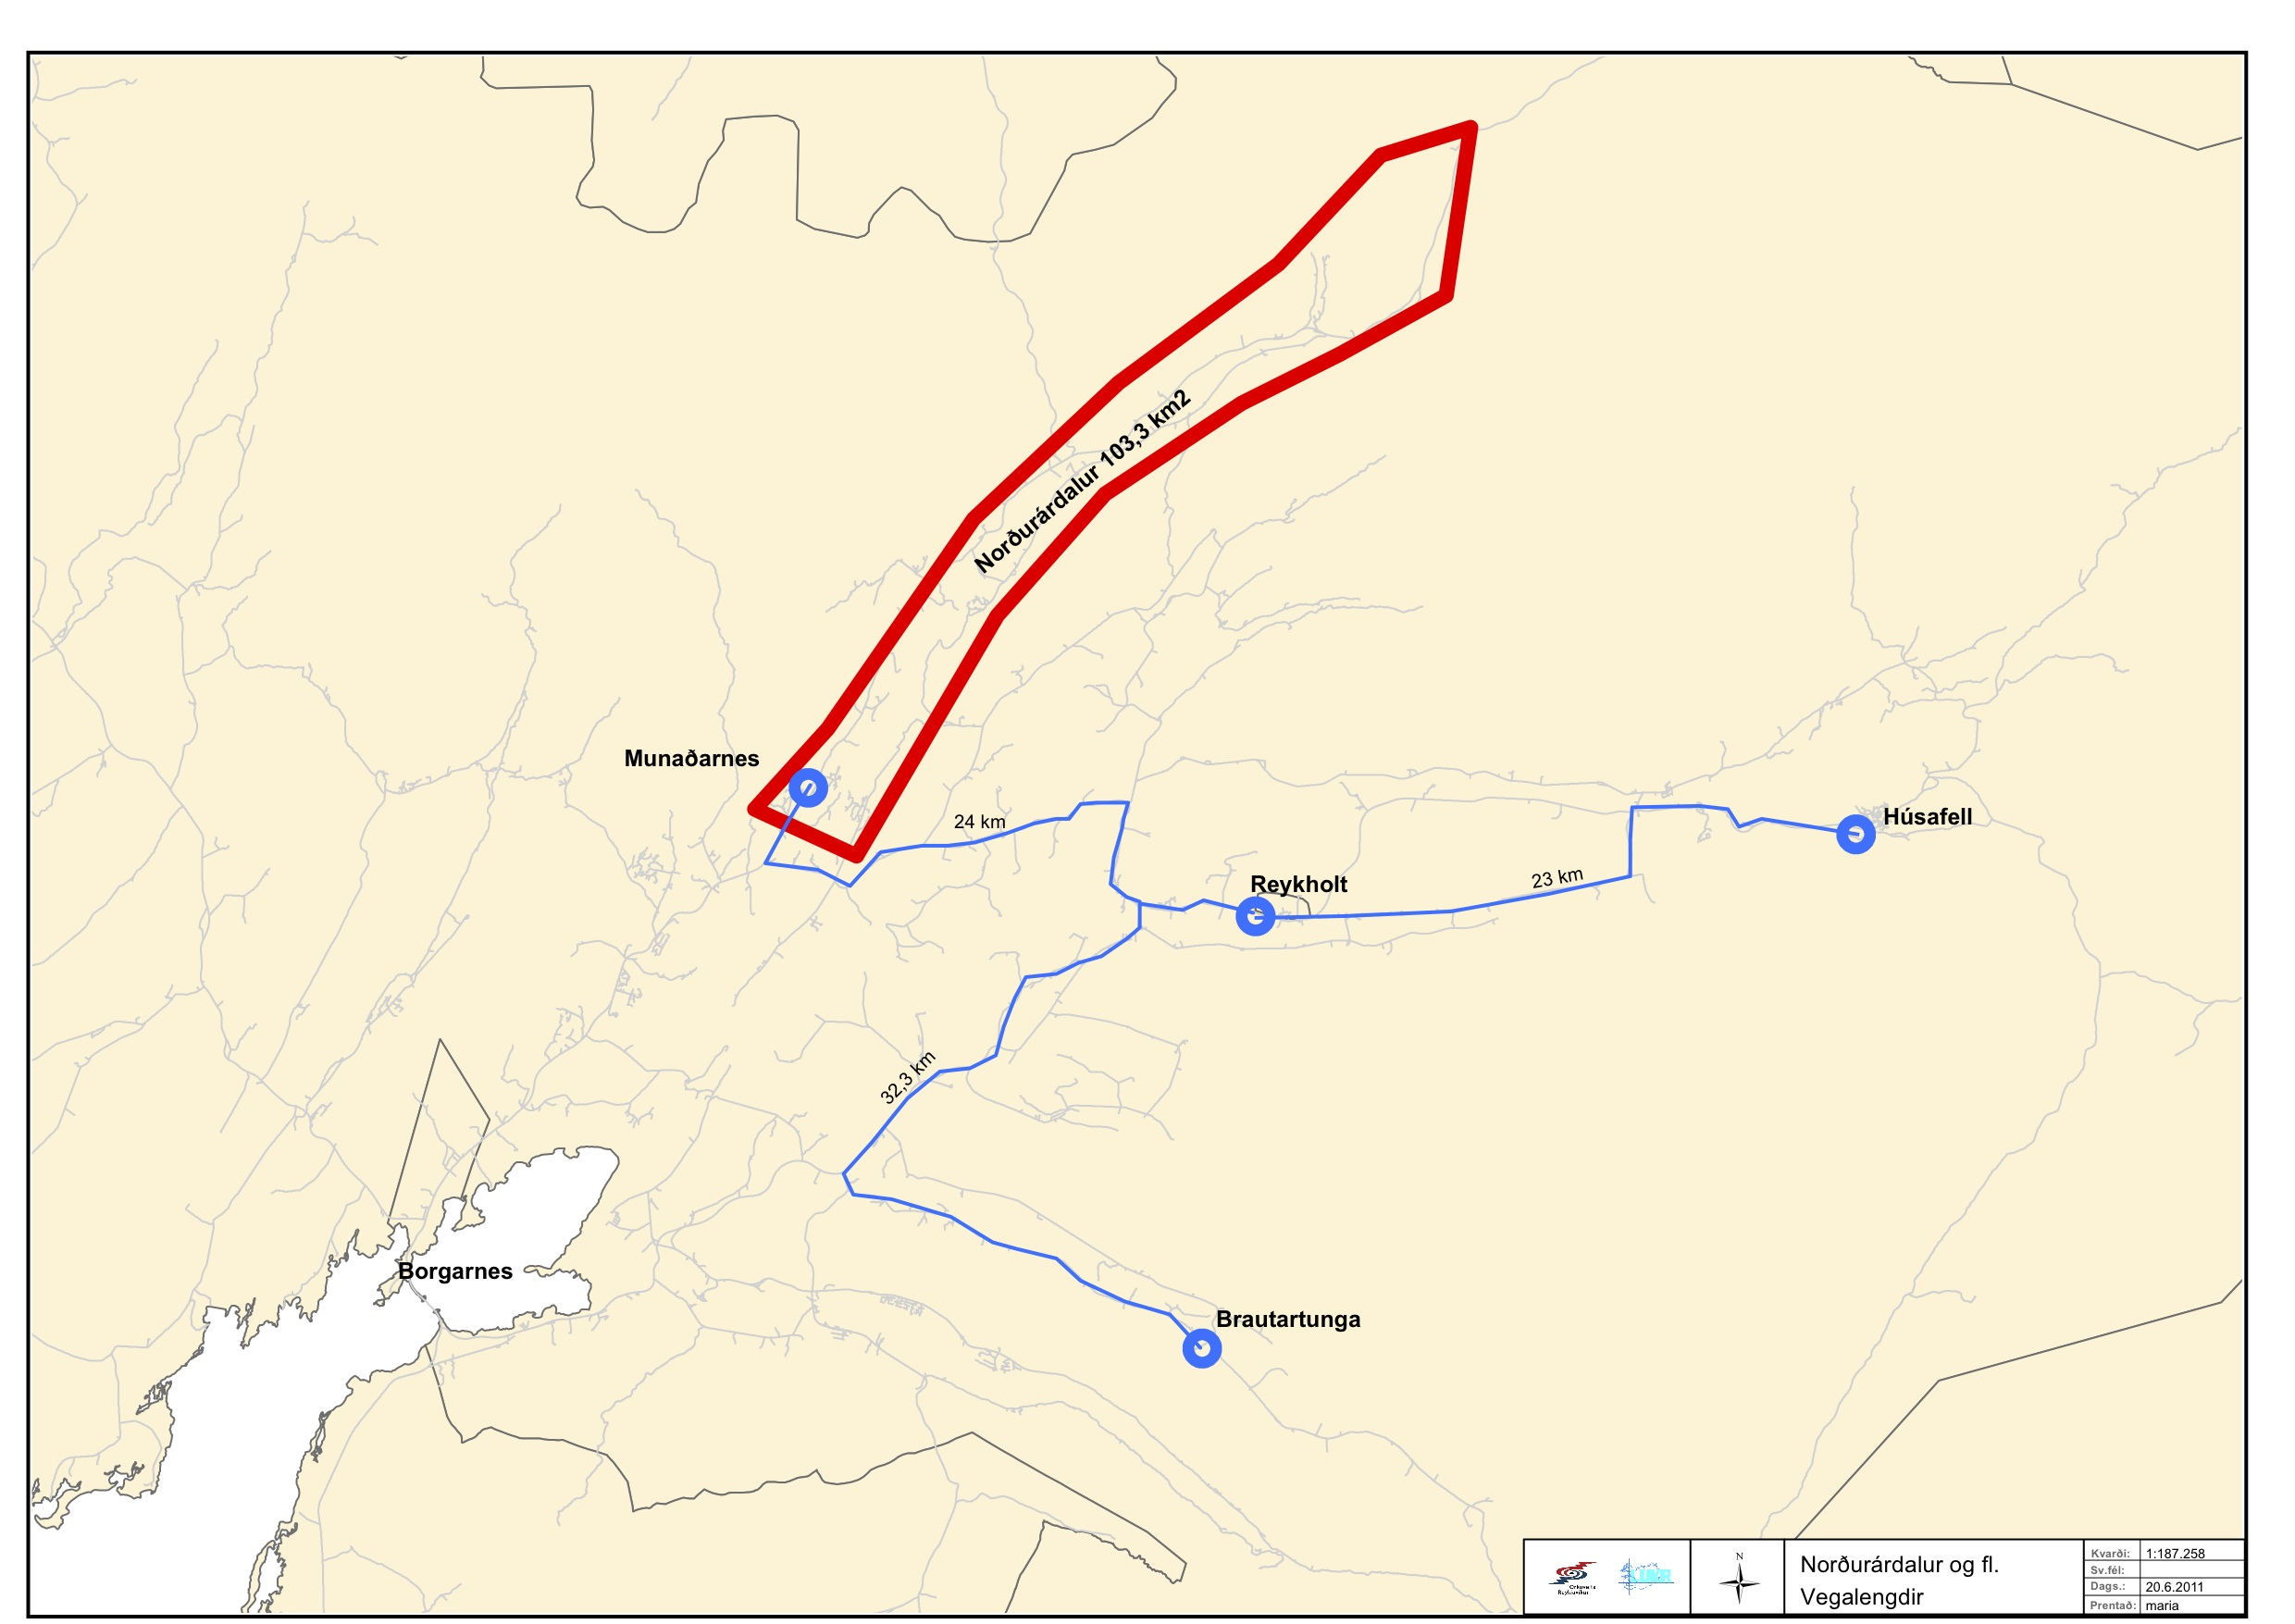
\includegraphics[width=6in]{nordu.jpg} 
%   \caption{ Borgarfjordur thermal field and Nordurardalur thermal system}
%   \label{fig:nordu}
%\end{figure}
%The Munardanes reservoir is situated in the Nordurardalur geothermal field. The later is located in west Iceland in the Borgarfjordur thermal field situated in the Borgarfjordur region. The Borgarfjordur thermal field is the largest low temperature geothermal field in Iceland. It comprises known thermal systems such as the Reykholt thermal system, the Bear thermal system, the Brautartunga thermal system, England thermal system, and the Husafell thermal system (Johannesson et al. 1980, Gunnlaugsson 1980). The natural discharge of the Borgarfjordur thermal system also called the Reykholtsdalur thermal system is estimated to 450$l/s$ of boiling water (Georgsson et al. 1984).  Within the Borgarfjordur thermal field, the Reykholf thermal system is by fare the largest thermal system with a total discharge of 400$l/s$ (Georgsson et al. 1980). The Nordurardalur thermal system is located north-west to the five major thermals systems mention above. It is a N-W long band of about 103 $km^{2}$ .
%
%\subsection{Geological setting}
%\begin{figure}[htbp] %  figure placement: here, top, bottom, or page
%   \centering
%   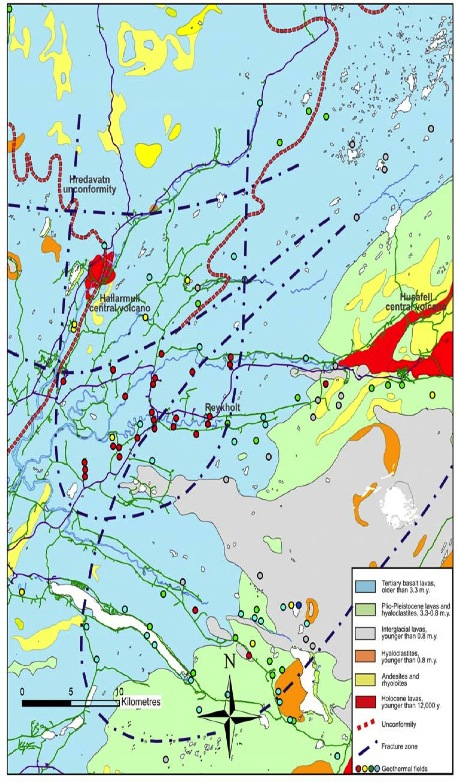
\includegraphics[width=4in]{bgeo.jpg} 
%   \caption{Geological map of Borgarfjordur thermal field}
%   \label{fig:bgeo}
%\end{figure}
%
%Upper tertiary ($>$3.3 Myr) basaltic lava flow constitute the basement of the Borgarfjordur region. This lava flow is characterised by a uniform lithology, either uniform texture or composition. The oldest rock being 14-15 Myrs. The bulk of this tertiary lava flow is made of tholeiites basaltic rock separated by minor clastic interbeds (Saemundsson 1979). The tholeiites basaltic lava pile is characterized by its content in sodium which is less than other basaltic rock. The Borgarfjordur thermal field is bounded from the east by the western volcanic rift zone and the snaefellnes volcanic zone from the west. The later present little or no rifting. Those two volcanic zones represent the origin of the tertiary lava flow.  However, the tholeiites content of the lava flow suggest that the lava flow is predominantly from the Sneafellsnes volcanic flank zone. \\
%\\
% Both unconformity and anticline structures are visible in the region. The later formed from rift relocation (Saemundsson, 1967). Recall that an anticline is defined as layers of sedimentary rock having the oldest strata in its core and forming a convex shape. An unconformity is a planar structure indicating a discontinuity in a geologicale structure due to erosive forces. The anticline axis is defined as the line of intersection of the perpendicular plane cutting the anticline in two symmetric parts. The Borganes anticline runs NE-SW (saemundsson 1977). The lava flow dip towards the Reykjanes-Langjokull rift zone to the east of the anticline axis. The Hredavatn unconformity is situated in north of Hredavatn lake. This unconformity indicate intense erosive forces acting in the borgarfjordur region.
%
%\subsection{Geophysical and hydrological setting}
%
%The geophysics of the region is characterised by the volcanism, the tectonic and the different forces affecting the earth crustal structure. The region is located between the Sneafellsnes volcanic flank and the Reykjanes-Langjokull volcanic rift. The later is made of the Reykjanes peninsula and the Western volcanic zone. The Reykjanes-Lanjokull rift is characterised by faulting resulting from tensional stress in the earth crust.  The Nordurardalur geothermal system is confined within the WNW-ESE, N-S  fractures zone   and between the Hradavatn unconformity and the Borganes anticline. An extinct central volcano is sitting within the Nordurardalur thermal system.\\
%The resistivity in Nordurardalur alternate between 20 and 100 $\Omega m$.  The 20 $\Omega m$ resistivity part is located in the lowest part of the Nordurardalur band and quickly 
%increase to 60 and 100 as we move North east. The value alternate to 30-40 then decrease to 20 before increasing to about 30 $\Omega m$.\\
%\\
%The geothermal water is of meteoric origin which as fallen as precipitation on the highland. The water percolate through fractures cracks or others pathways through the earth and is heated by regional heat flow. The flow pattern can be infer base on preview studies done in the main thermal systems in Borgafjordur. The Northeasterly faults are the main channels for the Nordurardalur thermal system and the seismicity in the region allows fractures to serve as flow path. The recharge zone is the Arnarvatnsheidi highland and the flow pattern is 
%
%\subsection{Proposed conceptual model of Borgarfjordur thermal filed}
%\begin{figure}[htbp] %  figure placement: here, top, bottom, or page
%   \centering
%   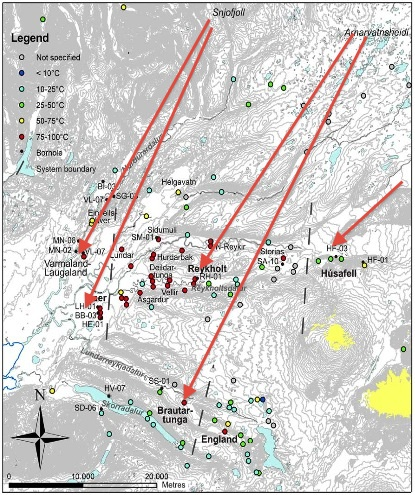
\includegraphics[width=5in]{flowp.jpg} 
%   \caption{Production well in Borgarfjordur thermal field with flow patterns of the main thermal systems}
%   \label{fig:flowp}
%\end{figure}
%Figure (\ref{fig:flowp}) indicates the flow patterns of the main thermal system in Borgarfjordur thermal field. The Reykholt and the Brautartungar thermal field recharge zone is located in the Arnarvatnsheidi high land. The Husafell thermal system recharge zone is located east to the Arnarvatnsheidi high land. For those tree systems, the easterly and north easterly faults and fractures allows the meteoric water to percolate at depth, acting as flow channels. The Nordurardalur system can be seen as a part of the Bear thermal system. The recharge zone is situated in the surrounding  of Snjofjoll, latitude 64 Degree 59 $mn$ $N$, longitude 21 Degree 11 $mn$ W. The $NS$ fractures act as flow channels, where the water flows by the Hallarmuli extinct central volcanoes. \\
%\\
%Heat is transfer by conduction through the earth crust from the Snaefellsnes volcanic flank and the Reykjaness-Langjokull volcanic rift zone. Heat is convected by the hot water though the fracture and fault systems at depth. The integrity of the fracture/fault system are maintain by the seismicity in the region. They also act as barriers zone. The salinity of water is the highest in the Bear thermal system as well as in the Nordurardalur system. As we move away from the Bear system the salinity decrease, being the lowest in Husafell thermal system.
%

%%%%%%%%%%%%%%%%%%%%%%%%%%%%%%%%%%%%%%%%%%%%%%%%%%%%%%%%%%

\subsection{Lumped parameter modelling of well $MN 08$ in Munadarnes in Nordurardalur}
Well $MN 8$ was drilled in 2003 east of the summer house lacerated in Munadarnes. The  $900 m$ deep low temperature well own by Reykjavik Energy was drilled after a survey revealed a temperature gradient of $250\,^{\circ}{\rm c}/km$ \cite{Hjartarson2003}. Testing and measurement of the well from February to March 2003 revealed that the temperature of the well is approximate $ 90\,^{\circ}{\rm c}$ and the main main feed zone is located at about $440 m$ \cite{Hjartarson2003}.\\


\begin{figure}[H] %  figure placement: here, top, bottom, or page
   \centering
   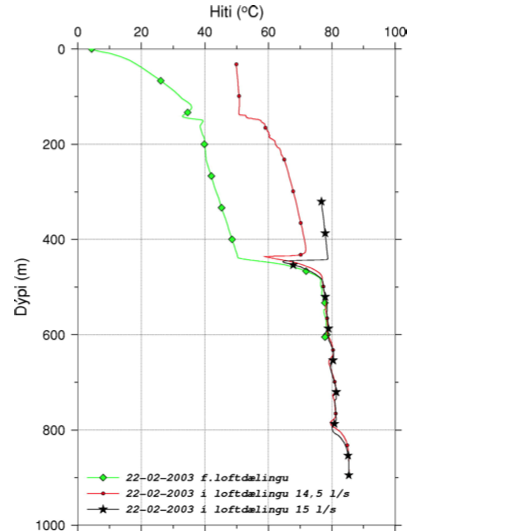
\includegraphics[width=4in]{tme.png} 
   \caption{Temperature measurement in well $MN 8$ \cite{Hjartarson2003}}
   \label{fig:example}
\end{figure}

Water level, pressure, temperature, production rate were monitored from January 2008 to December 2010. The well was initially drilled in 2003 with an initial water level of $35 m$. The first data set was rearrange by eliminating outliers, that is data points that are numerically distant from the rest of the data. The new data set was however still spread out.  Despite the spreading we  obtain a satisfactory  two tanks open model which was later used for future prediction. 

\subsubsection{Data processing and simulation}
The data obtained was very spread out. One possible explanation was that the data was contaminated by outliers.

\begin{table}[H]
	\begin{center}
		\begin{tabular}{|c|c|c|r|}
		\hline
			water level in $(m)$ & production in $(l/s)$ & date in $(YYY/mm/dd)$& time in $(hh:mm)$  \\ \hline
			$118.8$ &$8.8$  &$2010/03/29$  & $11:23$      \\ 
			$83.6$ & $7.1$ & $2010/01/06$  & $12:09$     \\ 
			$78.6$ &$8.4$ & $2009/12/01$   & $13:50$    \\ 
			$76.6$ &$8.4$ & $2010/02/15$    & $13:33$   \\ 
			$68.6$&$5.2$   & $2009/02/11$    & $10:20 $ \\ 
			$68.6$&$7.3$   & $2010/11/29$    & $14:22 $ \\ 
			$66.6$&$3$   & $2009/10/19$    & $9:40 $ \\ 
			$66.6$&$9$   & $2010/03/22$    & $13:55 $ \\ 
			$66.6$&$9$   & $2010/03/24$    & $20:09 $ \\ 

			\hline
		\end{tabular}
		\caption{Outliers removed from the simulated data}
		\label{tab:out}
	\end{center}
\end{table}


\begin{figure}[H] %  figure placement: here, top, bottom, or page
   \centering
   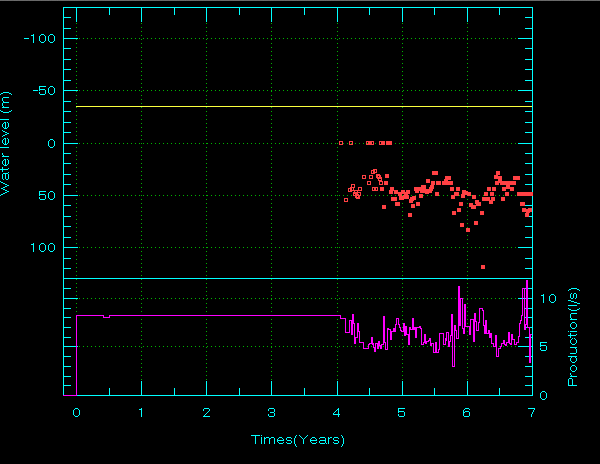
\includegraphics[width=4in]{idata.png}  
   \caption{Original data set}
   \label{fig:data}
\end{figure}

\begin{figure}[H] %  figure placement: here, top, bottom, or page
   \centering
   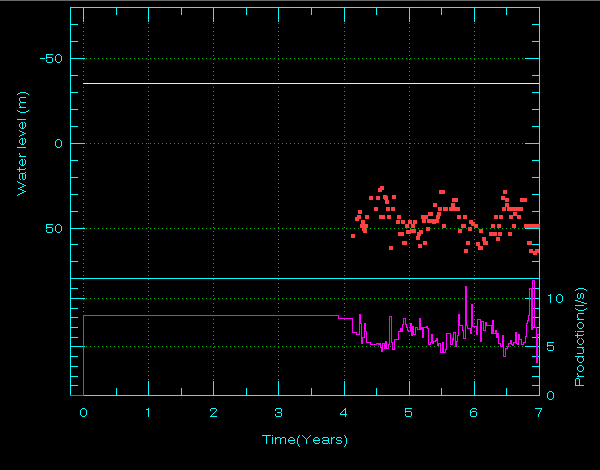
\includegraphics[width=4in]{ndata.png}  
   \caption{Data set obtained after removing the outliers in table \ref{tab:out} }
   \label{fig:data}
\end{figure}

\begin{figure}[H] %  figure placement: here, top, bottom, or page
   \centering
   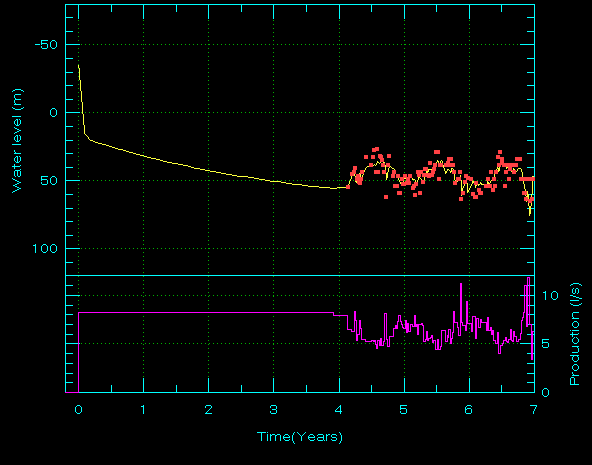
\includegraphics[width=4in]{twoto.png}  
   \caption{two tanks open model simulation }
   \label{fig:to}
\end{figure}




\begin{table}[H]%
\label{model}\centering 

\begin{tabular}{|c|l|c|c|c|}
\hline                                         
 Model number                 & 1           & 2         & 3  & 4        \\ %\toprule
\hline
Number of tanks              & 1           & 1        & 2   & 2 \\  %\midrule
\hline
Number of parameters  & 2           & 4        & 6     &  8   \\
\hline
Model types                     &Closed &Open& Closed & Open\\
\hline
$A_{1} $                           & 0    & 10.14  & 10.85 &17.8979            \\
\hline
$L_{1}$                            &  0      &  0.8   &  1.16& 2.82     \\
\hline
$A_{2}$                            &    0   &      0      & 0    &  0.17      \\
\hline
$L_{2}$                            &    0       & 0     & 0  & 0.025 \\
\hline
$B$  $(10^{-3})$              & 154.4  & 0  &  41.3 & 0 \\
\hline
$\kappa_{1} $                 & 1741.4 & 26.52& 24.68&14.88   \\
\hline
$\kappa_{2} $                 &0  & 0  & 6487.2&   1593.36        \\
\hline
$\kappa_{3}$                &   0 &   0   & 0 & 0 \\ 
\hline
$\sigma_{1}(10^{-6})$ &0 &  8     &  10.83& 16.8         \\
\hline
$\sigma_{2}(10^{-6})$  &   0 &   0&  0      &  15.2     \\
\hline
$RMS(m)$                       & 12.26 & 7.46 &   6.65 & 5.91           \\  %\bottomrule
\hline
$STD(m)$                          &12.31 &7.52 & 6.73&6.01   \\
\hline
$R^{2} (\%)$                      &0.00  &30.6  &44.88 & 56.46\\     
\hline  
\end{tabular}
\caption{Parameters of the lumped models for the production well $MN 8$ in Munardanes}
\label{tab:re}
\end{table}  



\begin{table}[H]%

\label{model}\centering 

\begin{tabular}{|c|l|}
\hline                                         
 Porosity $\phi$                 & 0.15        \\ %\toprule
\hline
depth $H (m)$              & 900       \\  %\midrule
\hline
gravity $(m/s^{-2})$  & 9.81        \\
\hline
Water compressibility  $C_{w} ( 10^{-10} Pa^{-1})$ & 4.6534 \\
\hline
Rock compressibility  $C_{r} (10^{-10} Pa^{-1})$ &3.3          \\
\hline
$s_{c} ( 10^{-7} kg/m^{3}Pa)$ &  3.4        \\
\hline
$s ( 10^{-5}kg/m^{3}Pa)$       &    1.7         \\
\hline  
\end{tabular}
\caption{Storativity estimation for  well $MN 8$ in Munardanes}
\label{tab:st}
\end{table}  
If the reservoir was confined, it would cover an area of about $525.5 km^{2}$ which is too large compared to the geothermal field. On the other hand, in the  unconfined case, the total area for the reservoir is about $10.5 km^{2}$. We therefore conclude that the reservoir is unconfined, with an approximated area of $10.5 km^{2}$. The permeability is estimated at about $69.8$ $mDarcy$. 



\subsubsection{ Prediction with reinjection}
Based on the analytical pressure response given in equation (\ref{eq:o}), a 20  years future prediction is given for different production scenarios.
% The storativity for an unconfined and a confined geothermal reservoir was given in section 2. For an average temperature of 86 degree c table \ref{tab:st} gives the storativity for confined $(s_{c})$ and unconfined $(s)$ reservoir.
%
%\begin{table}[H]%
%
%\label{model}\centering 
%
%\begin{tabular}{|c|l|}
%\hline                                         
% Porosity $\phi$                 & 0.15        \\ %\toprule
%\hline
%depth $H (m)$              & 900       \\  %\midrule
%\hline
%gravity $(m/s^{-2})$  & 9.81        \\
%\hline
%Water compressibility  $C_{w} ( 10^{-10} Pa^{-1})$ & 4.6534 \\
%\hline
%Rock compressibility  $C_{r} (10^{-10} Pa^{-1})$ &3.3          \\
%\hline
%$s_{c} ( 10^{-7} kg/m^{3}Pa)$ &  3.4        \\
%\hline
%$s ( 10^{-5}kg/m^{3}Pa)$       &    1.7         \\
%\hline  
%\end{tabular}
%\caption{Storativity estimation for  well $MN 8$ in Munardanes}
%\label{tab:st}
%\end{table}  
%If the reservoir was confined, it would cover an area of about $525.5 km^{2}$ which is too large compared to the geothermal field. On the other hand, in the  unconfined case, the total area for the reservoir is about $10.5 km^{2}$. We therefore conclude that the reservoir is unconfined, with an approximated area of $10.5 km^{2}$. The permeability is estimated at about $6.98.10^{-10} m^{2}$ or $69.8$ $mDarcy$. Based on the analytical pressure response given in equation (\ref{eq:o}), a 20  years future prediction is given in figure \ref{fig:f} for different production scenario.


\begin{figure}[H] %  figure placement: here, top, bottom, or page
   \centering
   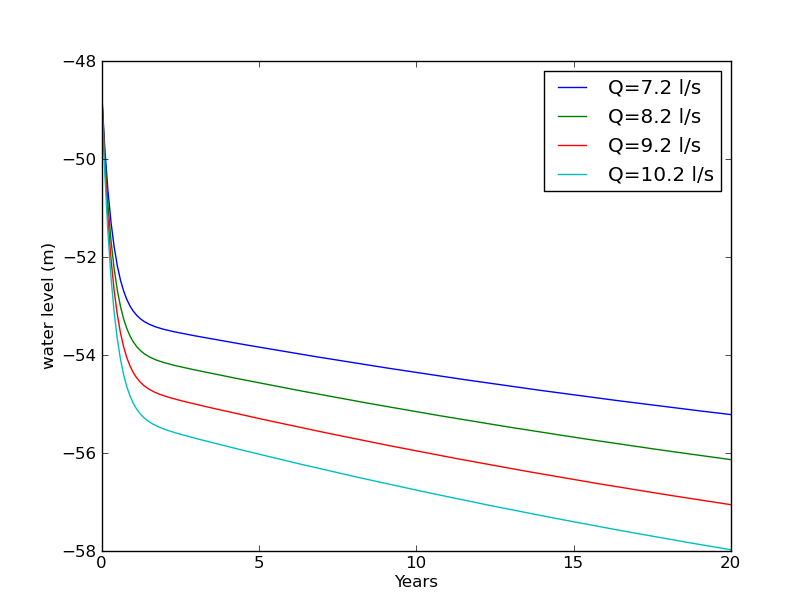
\includegraphics[width=4in]{future.png} 
   \caption{ 20 years future prediction from 2010, without reinjection}
   \label{fig:f}
\end{figure}

\begin{figure}[H] %  figure placement: here, top, bottom, or page
   \centering
   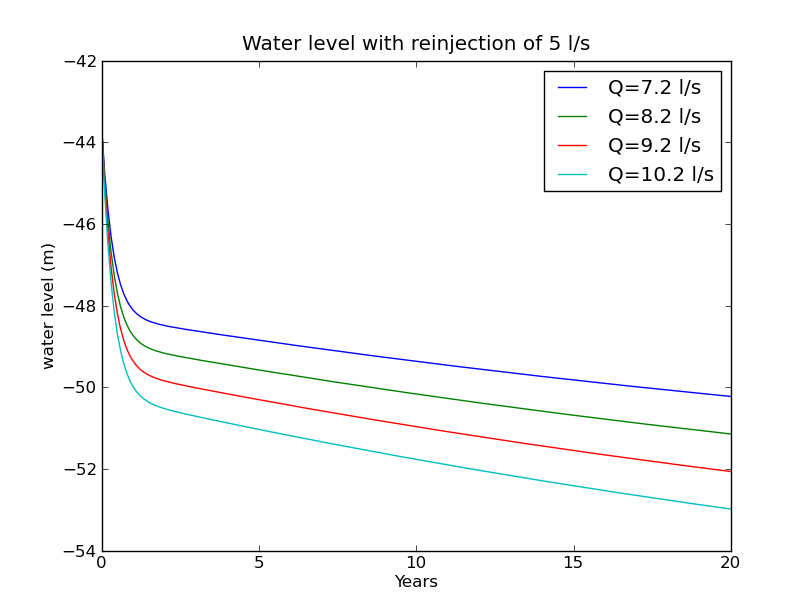
\includegraphics[width=4in]{r5.png} 
   \caption{20 years production with reinjection scenario for 5 $l/s$ injection rate at the start of production}
   \label{fig:r5}
\end{figure}

\begin{figure}[H] %  figure placement: here, top, bottom, or page
   \centering
   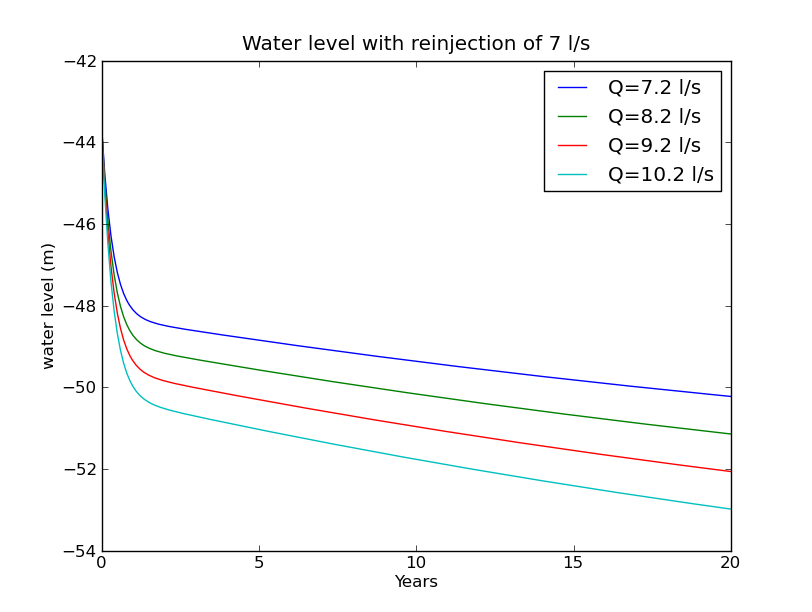
\includegraphics[width=4in]{r7.png} 
   \caption{20 years production with reinjection scenario for 7 $l/s$ injection rate at the start of production}
   \label{fig:r7}
\end{figure}

\begin{figure}[H] %  figure placement: here, top, bottom, or page
   \centering
   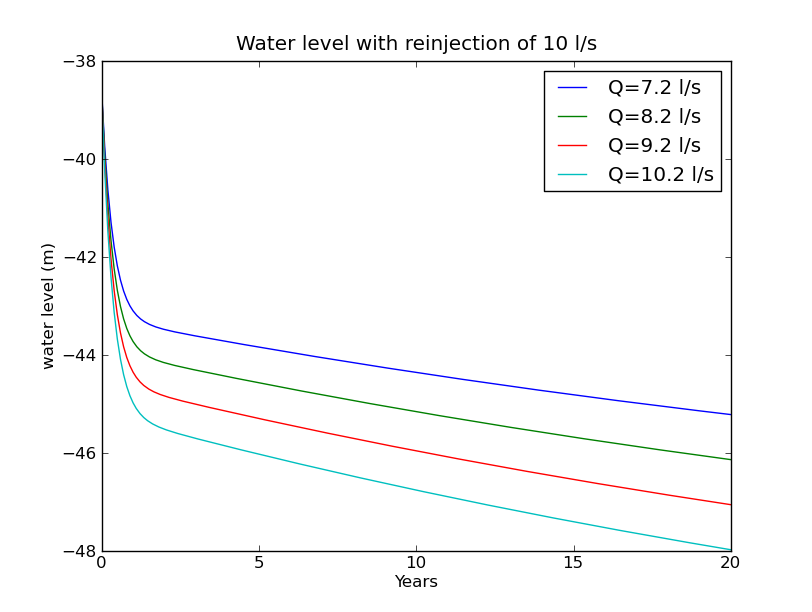
\includegraphics[width=4in]{10ls.png} 
   \caption{ 20 years production with reinjection scenario for 10 $l/s$ injection rate at the start of production}
   \label{fig:10ls}
\end{figure}


Figure \ref{fig:f} shows a 20 years prediction with production rate of $7.2$ $l/s$, $8.2$ $l/s$, $9.2$ $l/s$ and $10.2$ $l/s$.  Figure \ref{fig:r5}, \ref{fig:r7} and \ref{fig:10ls} shows the change in water level over a period of 20 years with three injection scenarios of water at 5, 7 and $10$ $l/s$ reinjection rate. The reinjection scenarios assumed that reinjection started at the beginning of of 2004. The minimum and maximum production rate are assumed to be $7.2$ $l/s$, $10.2$ $l/s$ respectively. As seen water leveel increases significantly with injection. However due to the cold nature of the injected water some cooling can be induce.\\
\\
\subsubsection{ Location of injection well and cooling of production well}\\

Based of a theoretical model of a one dimension flow channel, along a fracture zone, The temperature of a production well is given by \cite{Axelsson2005}:

\begin{equation}\label{eq:cool}
T(t) = T_{0}-\frac{q}{Q}(T_{0}-T_{i})\left (  1-\erf\left(    \frac{kxh}{c_{w}q\sqrt{\kappa(t-x/\beta)}}}       \right)        \right)
\end{equation}
with $T(t)$ the production fluid temperature, $T_{0}$ the undisturbed reservoir temperature, $T_{i}$ the injection temperature, $q$ and $Q$ the rate of injection and production respectively, $k$ the thermal conduction of the reservoir rock, $\kappa$ the thermal diffusivity, $x$ the distance between injection and production wells and
\begin{equation}
\beta = \frac{qc_{w}}{<\rho c>_{f}hb} \nonumber
\end{equation}
with 
\begin{equation}
<\rho c>_{f} =\rho_{w}c_{w}+\rho_{r}c_{r}(1-\phi) \nonumber
\end{equation}
the volumetric heat capacity of the material in the flow channe. $\rho$ and $c$ are density and heat capacity respectively, with indices $w$ and $r$ standing for water and rock.

\begin{figure}[H] %  figure placement: here, top, bottom, or page
   \centering
   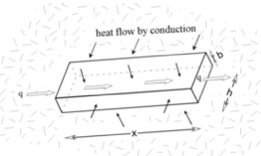
\includegraphics[width=4in]{fc.png} 
   \caption{model of flow channel for cooling of production well during injection \cite{Axelsson2005}}
   \label{fig:fc}
\end{figure}

Assume a one dimensional channel with $h = 29$ $m$, $b=7$ $m$ and porosity $\phi = 0.15$. The injection water temperature is $T_{i}=20\,^{\circ}{\rm c}$ and the reservoir temperature $T_{0}=86\,^{\circ}{\rm c}$. The thermal conductivity $k=2$. The specific heat capacity and the density are given by Stoppa et. al as a function of temperature \cite{Waj05}. The theoretical cooling of well $MN 08$ in Munadarnes during a 10 years reinjection scenario is given bellow:


\begin{figure}[H] %  figure placement: here, top, bottom, or page
   \centering
   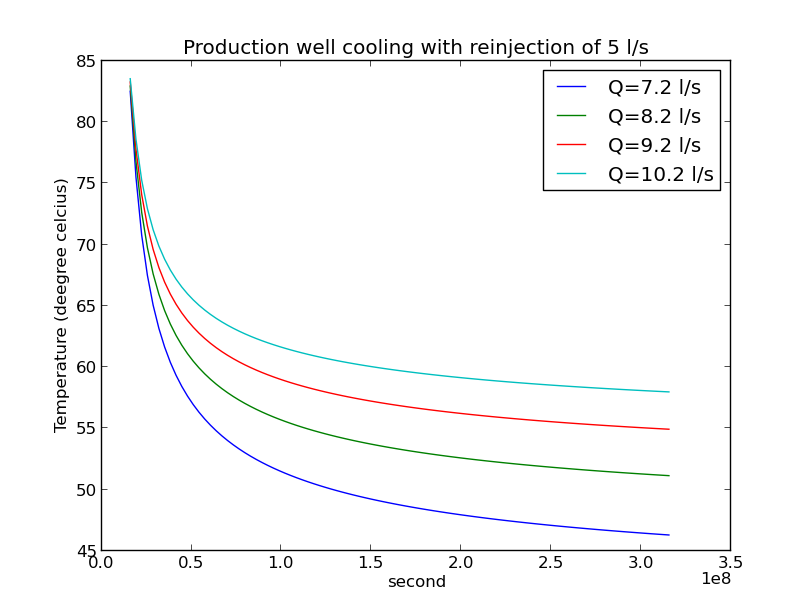
\includegraphics[width=4in]{5ls500m.png} 
   \caption{Production well cooling for injection well located at $500$ $m$ from production well. Injection rate 5 $l/s$}
   \label{fig:one}
\end{figure}

\begin{figure}[H] %  figure placement: here, top, bottom, or page
   \centering
   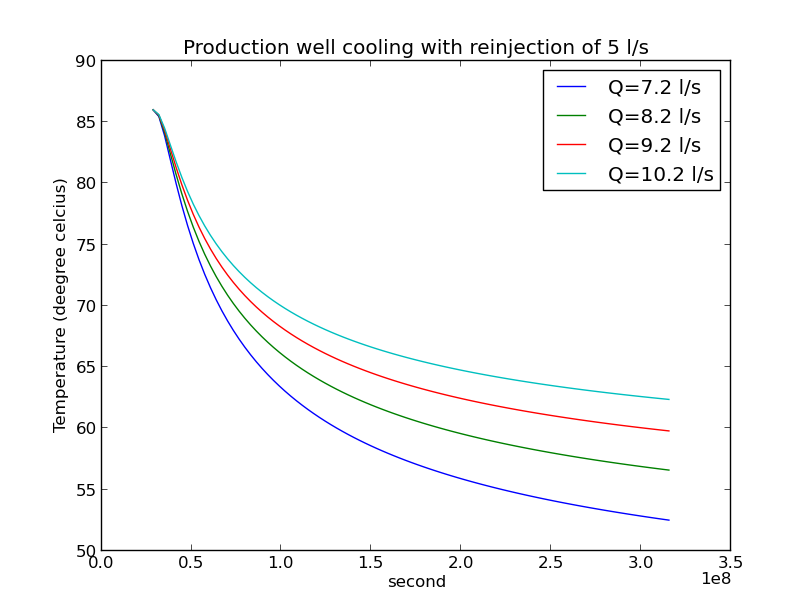
\includegraphics[width=4in]{5ls1km.png} 
   \caption{Production well cooling for injection well located at $1$ $km$ from production well. Injection rate 5 $l/s$}
   \label{fig:two}
\end{figure}

\begin{figure}[H] %  figure placement: here, top, bottom, or page
   \centering
   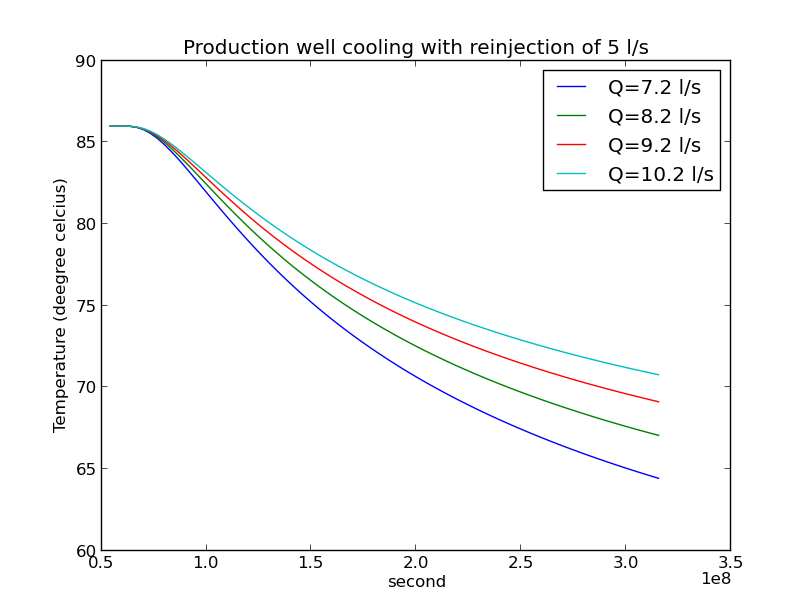
\includegraphics[width=4in]{5ls2km.png} 
   \caption{Production well cooling for injection well located at $2$ $km$ from production well. Injection rate 5 $l/s$}
   \label{fig:three}
\end{figure}


\begin{figure}[H] %  figure placement: here, top, bottom, or page
   \centering
   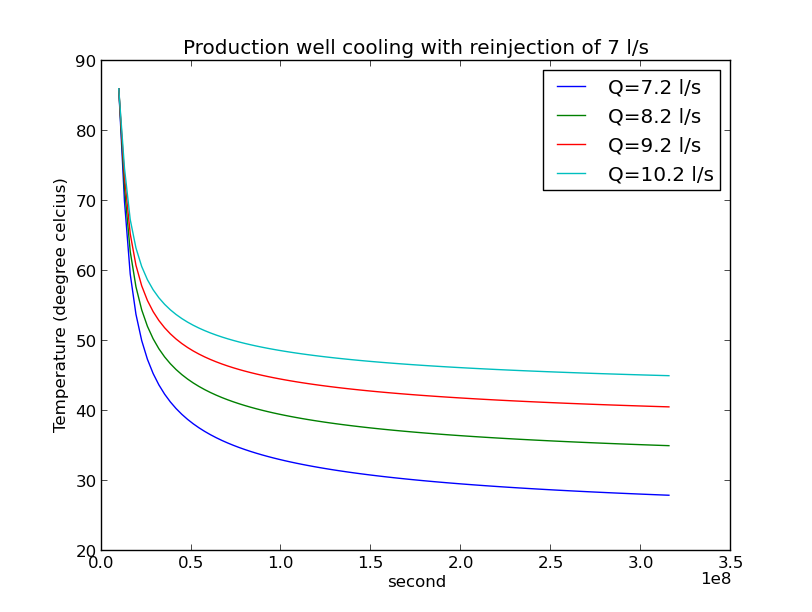
\includegraphics[width=4in]{7ls500m.png} 
   \caption{Production well cooling for injection well located at $500$ $m$ from production well. Injection rate 7 $l/s$}
   \label{fig:four}
\end{figure}

\begin{figure}[H] %  figure placement: here, top, bottom, or page
   \centering
   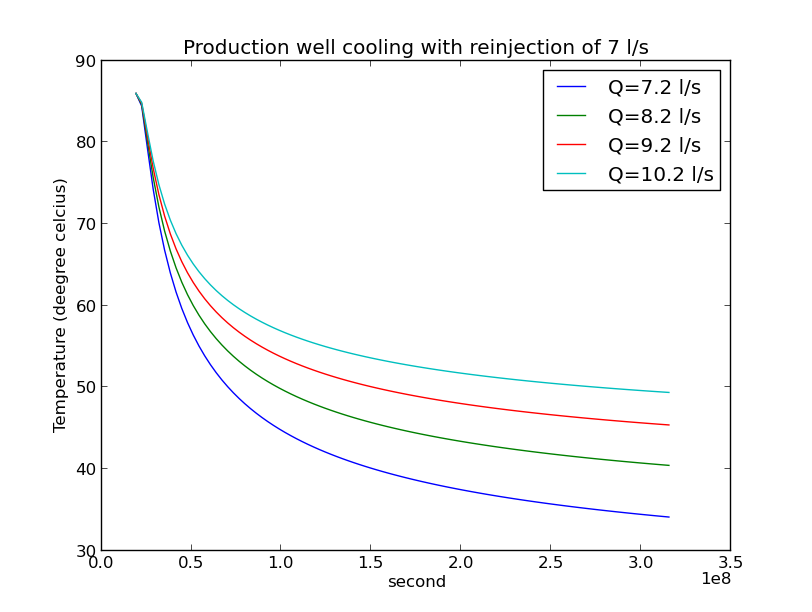
\includegraphics[width=4in]{7ls1km.png} 
   \caption{Production well cooling for injection well located at $1$ $km$ from production well. Injection rate 7 $l/s$}
   \label{fig:five}
\end{figure}

\begin{figure}[H] %  figure placement: here, top, bottom, or page
   \centering
   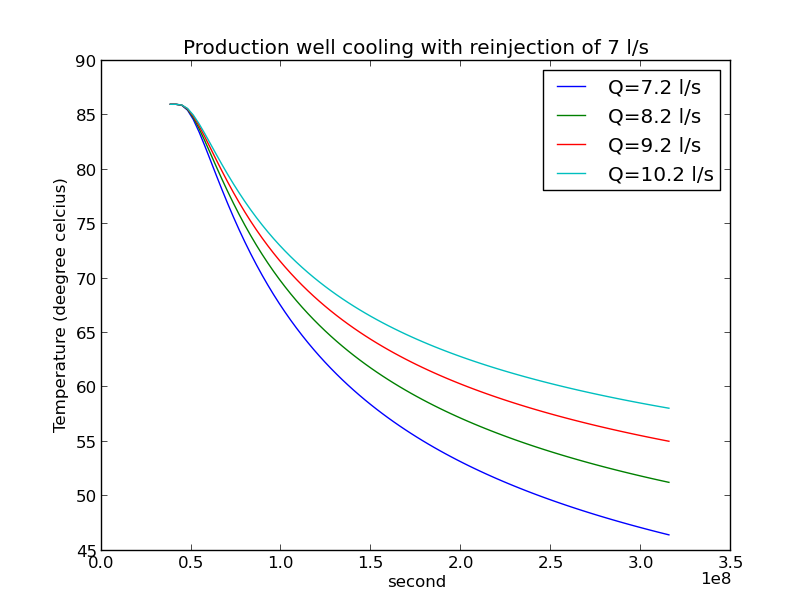
\includegraphics[width=4in]{7ls2km.png} 
   \caption{Production well cooling for injection well located at $2$ $km$ from production well. Injection rate 7 $l/s$}
   \label{fig:six}
\end{figure}
As seen from Figures \ref{fig:one} to \ref{fig:six} the temperature of the production well decrease when the injection well is closer to the production well. At a distance of 2 $km$ the cooling effect is attenuated. The production well temperature is lower for higher injection rate. As the production rate is increased so is the temperature of the production well during injection.




